\section{Mikrocontroller PIC16F84A}

Ein Mikrocontroller ist eine Art Mikrorechnersystem, bei welchem neben ROM und RAM auch Peripherieeinheiten wie Schnittstellen, Timer und Bussysteme auf einem einzigen Chip integriert sind.
Die Hauptanwendungsgebiete sind die Steuerungs-, Mess- und Regelungstechnik, sowie die Kommunikationstechnik und die Bildverarbeitung. Mikrocontroller sind in der Regel in Embedded Systems, in die Anwendung eingebettete Systeme, und somit in der Regel von au�en nicht sichtbar. Ebenso verf�gen sie, im Gegensatz zum PC, nicht �ber eine direkte Bedien- und Prorgrammierschnittstelle zum Benutzer. Sie werden in der Regel einmal programmiert und installiert.

Der PIC16F84 Mikrocontroller ist ein 8 Bit Mikrocontroller mit RISC-Architektur (Reduced-Instruction-Set-Computing). Es wird also auf komplexe Befehle verzichtet und mit jedem Befehl kann auf jedes Register zugegriffen werden. Der Mikrocontroller besitzt durch die eingesetzte Harvard-Architektur bis zu 14 Bit gro�e Befehle w�hrend die Gr��e des separaten Datenbusses nur 8 Bit betr�gt.

\begin{figure}[htb]
\centering
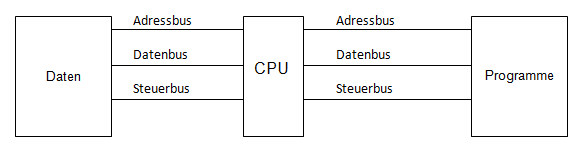
\includegraphics{Bilder/Harvard}
\caption{Harvard-Architektur}
\end{figure}

\newpage
Durch die Architektur ben�tigen fast alle Anweisungen nur einen Instruction Cycle (Abarbeitung eines Maschinenbefehls).
Der PIC16 besitzt einen Stack mit Speicherplatz f�r 8 Adressen sowie 2 externe und 2 interne Interrupt Quellen. Dar�ber hinaus besitzt der Pic16F ein gro�es Register, welches in zwei B�nke unterteilt ist. Das Umschalten der B�nke erfolgt im Programmcode. Die Speicherbereiche k�nnen auch direkt �ber ihre Registeradresse angesprochen werden.
